\documentclass[tikz,border=10pt]{standalone}
\usepackage{tikz}
\usetikzlibrary{shapes.multipart, shadows, positioning, arrows.meta, calc, backgrounds, decorations.pathreplacing}
\usepackage{newtxtext,newtxmath}
\usepackage{array} 

% --- 配色方案 ---
% 1. Seq Cst - Red
\definecolor{cSeqFill}{RGB}{255, 235, 238}
\definecolor{cSeqDraw}{RGB}{211, 47, 47}
\definecolor{cSeqText}{RGB}{183, 28, 28}

% 2. Acquire/Release - Amber/Orange
\definecolor{cAcqFill}{RGB}{255, 248, 225}
\definecolor{cAcqDraw}{RGB}{255, 160, 0}
\definecolor{cAcqText}{RGB}{230, 81, 0}

% 3. Relaxed - Green
\definecolor{cRelFill}{RGB}{232, 245, 233}
\definecolor{cRelDraw}{RGB}{56, 142, 60}
\definecolor{cRelText}{RGB}{27, 94, 32}

\begin{document}
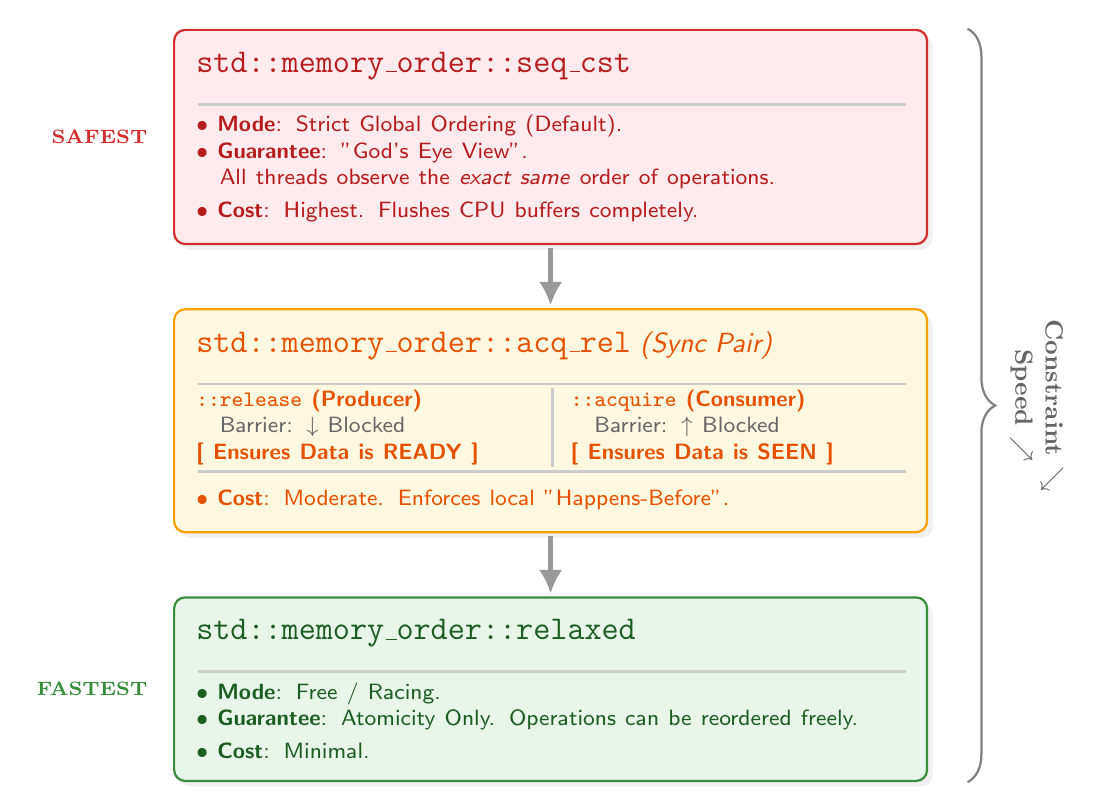
\begin{tikzpicture}[
	font=\sffamily,
	node distance=0.8cm, % 缩小卡片间距
	% 基础卡片样式
	card/.style={
			rectangle,
			rounded corners=4pt,
			thick,
			text width=9.0cm, % 宽度给足,防止换行挤压
			align=left,
			inner sep=8pt,    % 稍微减小内边距
			drop shadow={opacity=0.12, shadow xshift=2pt, shadow yshift=-2pt}
		},
	% 连线样式
	flowArrow/.style={
	draw=black!40,
	line width=2pt,
	-{Latex[length=3mm, width=3mm]},
	shorten >= 1pt, shorten <= 1pt
	},
	% 辅助分割线
	divLine/.style={
			draw=black!20,
			line width=1pt
		}
	]

	% =========================================================
	% 1. 顺序一致性 (Sequential Consistency)
	% =========================================================
	\node[card, draw=cSeqDraw, fill=cSeqFill, text=cSeqText] (seq) {
		\texttt{\textbf{\large std::memory\_order::seq\_cst}}

		\tikz \draw[divLine] (0,0) -- (9.0,0); % 分割线

		\footnotesize
		$\bullet$ \textbf{Mode}: Strict Global Ordering (Default).\\
		$\bullet$ \textbf{Guarantee}: "God's Eye View". \\
		\quad All threads observe the \textit{exact same} order of operations.\\
		$\bullet$ \textbf{Cost}: Highest. Flushes CPU buffers completely.
	};

	% =========================================================
	% 2. 获取/发布 (Acquire / Release) - 紧凑分栏
	% =========================================================
	\node[card, draw=cAcqDraw, fill=cAcqFill, text=cAcqText, below=of seq] (acq) {
		\texttt{\textbf{\large std::memory\_order::acq\_rel}} \textit{(Sync Pair)}

		\tikz \draw[divLine] (0,0) -- (9.0,0);

		\footnotesize
		% 定义列格式:左对齐,去除额外间距,中间插入淡灰色竖线
		\begin{tabular}{@{} >{\raggedright\arraybackslash}p{4.3cm} !{\color{black!20}\vrule width 1pt} >{\raggedright\arraybackslash}p{4.3cm} @{}}
			% --- Header ---
			\textbf{\texttt{::release} (Producer)}              & \textbf{\texttt{::acquire} (Consumer)}            \\

			% --- Body ---
			\quad \color{black!60}Barrier: $\downarrow$ Blocked & \quad \color{black!60}Barrier: $\uparrow$ Blocked \\

			% --- Key Concept (Be Seen / Be Ready) ---
			\textbf{[ Ensures Data is READY ]}                  & \textbf{[ Ensures Data is SEEN ]}
		\end{tabular}

		\tikz \draw[divLine] (0,0) -- (9.0,0);

		$\bullet$ \textbf{Cost}: Moderate. Enforces local "Happens-Before".
	};

	% =========================================================
	% 3. 松散序 (Relaxed)
	% =========================================================
	\node[card, draw=cRelDraw, fill=cRelFill, text=cRelText, below=of acq] (rel) {
		\texttt{\textbf{\large std::memory\_order::relaxed}}

		\tikz \draw[divLine] (0,0) -- (9.0,0);

		\footnotesize
		$\bullet$ \textbf{Mode}: Free / Racing.\\
		$\bullet$ \textbf{Guarantee}: Atomicity Only. Operations can be reordered freely.\\
		$\bullet$ \textbf{Cost}: Minimal.
	};

	% =========================================================
	% 4. 连线
	% =========================================================
	\draw[flowArrow] (seq) -- (acq);
	\draw[flowArrow] (acq) -- (rel);

	% =========================================================
	% 5. 右侧标尺
	% =========================================================
	\coordinate (topRight) at ($(seq.north east) + (0.5, 0)$);
	\coordinate (bottomRight) at ($(rel.south east) + (0.5, 0)$);

	\draw[decorate, decoration={brace, amplitude=10pt}, thick, black!50]
	(topRight) -- (bottomRight)
	node[midway, xshift=2.5em, rotate=-90, align=center, font=\bfseries\small, text=black!60]
	{Constraint $\searrow$ \\ Speed $\nearrow$};

	% 左侧标签
	\node[anchor=east, font=\bfseries\scriptsize, text=cSeqDraw] at ($(seq.west) + (-0.2,0)$) {SAFEST};
	\node[anchor=east, font=\bfseries\scriptsize, text=cRelDraw] at ($(rel.west) + (-0.2,0)$) {FASTEST};

\end{tikzpicture}
\end{document}